% ============================================================
%  MorphoHand v2: Expanded Proposal / Working Paper
%  No page limit — structured as an in-progress research document
%  with educational depth on all key concepts.
% ============================================================

\documentclass[journal]{IEEEtran}

\usepackage{cite}
\usepackage{amsmath,amssymb,amsfonts}
\usepackage{algorithm}
\usepackage{algorithmic}
\usepackage{graphicx}
\usepackage{textcomp}
\usepackage{xcolor}
\usepackage{booktabs}
\usepackage{multirow}
\usepackage{hyperref}
\usepackage{enumitem}
\usepackage{tikz}
\usepackage{pgfplots}
\pgfplotsset{compat=1.18}
\usetikzlibrary{
  arrows.meta, positioning, shapes.geometric, fit,
  backgrounds, decorations.pathreplacing, calc, patterns
}
\usepackage{tcolorbox}
\tcbuselibrary{skins, breakable}

% ── colour palette ───────────────────────────────────────────
\definecolor{mblue}{RGB}{31,119,180}
\definecolor{morange}{RGB}{255,127,14}
\definecolor{mgreen}{RGB}{44,160,44}
\definecolor{mred}{RGB}{214,39,40}
\definecolor{mpurple}{RGB}{148,103,189}
\definecolor{mgray}{RGB}{127,127,127}
\definecolor{heilgray}{RGB}{248,248,248}
\definecolor{notegray}{RGB}{240,244,250}

% ── callout box for Heilmeier ────────────────────────────────
\newtcolorbox{heilbox}{
  enhanced, breakable,
  colback=heilgray, colframe=mgray!80,
  fonttitle=\bfseries, title={Heilmeier Catechism},
  left=5pt, right=5pt, top=4pt, bottom=4pt,
  before upper={\small\setlength{\parskip}{3pt}},
}

% ── callout box for design notes / background explanations ──
\newtcolorbox{notebox}[1][Note]{
  enhanced, breakable,
  colback=notegray, colframe=mblue!60,
  fonttitle=\bfseries\small, title={#1},
  left=4pt, right=4pt, top=3pt, bottom=3pt,
  before upper={\small},
}

\def\BibTeX{{\rm B\kern-.05em{\sc i\kern-.025em b}\kern-.08em
    T\kern-.1667em\lower.7ex\hbox{E}\kern-.125emX}}

\newcommand{\btheta}{\boldsymbol{\theta}}
\newcommand{\bq}{\mathbf{q}}
\newcommand{\bw}{\mathbf{w}}
\newcommand{\cO}{\mathcal{O}}
\newcommand{\cQ}{\mathcal{Q}}
\newcommand{\cA}{\mathcal{A}}
\newcommand{\R}{\mathbb{R}}
\newcommand{\eps}{\epsilon}

% ============================================================
\begin{document}
% ============================================================

\title{A Reconfigurable Hand Platform
for Physical Validation of Simulation-Optimized Morphologies}
% \large{\textit{(Working Paper / Research Proposal --- v2)}}}

\author{
  \IEEEauthorblockN{William Xie} \\
  \IEEEauthorblockA{
    University of Colorado Boulder\\
    \texttt{william.xie@colorado.edu}
  }
}

\maketitle

% ============================================================
%  HEILMEIER CATECHISM
% ============================================================
\begin{heilbox}
\textbf{The Heilmeier Catechism} is a set of questions originally developed at DARPA to
evaluate whether a research proposal is clear, honest, and grounded.
We answer them here in plain language before the technical material.

\smallskip
\textbf{H1. What are you trying to do?}\\
We want to know what shape a robot hand should be to grasp a given set of objects as well
as possible.
We believe different sets of objects require structurally different hands, and we want to
prove this with hardware measurements rather than just simulation.

\smallskip
\textbf{H2. How is it done today, and what are the limits of current practice?}\\
Researchers either design hands by intuition and test through expensive fabrication iterations,
or optimize in simulation and physically build one or a few winning candidates.
Neither approach lets you compare many different hand shapes on the same physical hardware
under identical conditions, so the simulation-to-reality gap for \emph{morphology} itself
remains largely unmeasured.

\smallskip
\textbf{H3. What is new in your approach and why do you think it will be successful?}\\
We build a single motorized platform that can physically reconfigure into millions of
distinct 3-finger hand shapes without disassembly.
Paired with a quality-diversity optimizer in simulation that explores how performance
varies \emph{across} morphology space rather than just finding the single best shape,
we can test many designs on real hardware in one session, eliminating fabrication variance
as a confound.

\smallskip
\textbf{H4. Who cares? If you are successful, what difference will it make?}\\
Anyone designing a robot hand for a known task distribution---industrial picking,
agricultural harvesting, assistive devices---needs principled morphology guidance.
Success would establish the first hardware-grounded methodology for morphology validation,
and provide empirical evidence that task-specific hand design genuinely outperforms
general-purpose design in identifiable ways.

\smallskip
\textbf{H5. What are the risks?}\\
The simulation-to-reality gap for contact mechanics may cause simulated quality rankings
to disagree with physical outcomes; the reconfigurable platform introduces mechanical
backlash and compliance not present in a purpose-built hand, which could confound measurements.

\smallskip
\textbf{H6. How much will it cost?}\\
Hardware (motors, rails, custom mounts, fingertip tooling): approximately \$8{,}000--\$15{,}000.
Compute (GPU time for parallel simulation and quality-diversity search): \$5{,}000--\$10{,}000
in cloud credits or equivalent on-premise GPU time.

\smallskip
\textbf{H7. How long will it take?}\\
Eighteen to twenty-four months: six months for hardware design and fabrication,
six months for the simulation and optimization framework, six months for experiments
and writing.

\smallskip
\textbf{H8. What are the mid-term and final ``exams'' to check for success?}\\
\emph{Mid-term}: the platform reliably realizes at least 50 distinct morphology configurations
and records repeatable grasp outcomes on a 20-object set.
\emph{Final}: simulation-predicted morphology rankings show statistically significant rank
correlation with physical hardware rankings ($\tau > 0.7$, Kendall's $\tau$), and we
demonstrate that object-set-specific optimal morphologies differ significantly from the
morphology optimized for the full set.
\end{heilbox}

% ============================================================
\begin{abstract}
Robotic hand design is a morphology optimization problem: the placement, orientation,
and link lengths of fingers determine which grasps are reachable and how stable they are
across a distribution of target objects.
Despite decades of research on dexterous hands, the field lacks a principled,
hardware-grounded method for comparing many different morphologies under identical physical
conditions.
Existing practice either builds one or a few physical prototypes and tests them, or
optimizes geometry in simulation and fabricates the winning design, leaving the
simulation-to-reality gap for \emph{morphology} (as opposed to control policy)
largely uncharacterized.

We propose \textbf{MorphoHand}, an 18-degree-of-freedom reconfigurable robotic hand
designed as a physical oracle for simulation-based morphology optimization.
Three fingers---thumb, index, and middle---each mount on a 2-DOF Cartesian gantry for
continuous repositioning in the palm plane, with additional motorized yaw,
MCP flex/extension, proximal phalange length adjustment via an internal linear actuator,
and PIP flex/extension, yielding six independent degrees of freedom per finger.
Hot-swap fingertip mounts allow task-specific contact geometry to be changed in under
30 seconds per finger.

On the simulation side, we develop a Quality-Diversity (QD) optimization pipeline
using MAP-Elites as the outer morphology search algorithm and a differentiable Grasp
Wrench Space (GWS) metric as the inner grasp quality oracle.
Rather than searching for a single optimal hand shape, MAP-Elites builds an \emph{archive}
that illuminates how quality varies continuously across the morphology design space---a
representation that directly encodes which morphologies are good for which kinds of objects.

The central scientific question we aim to answer is: \emph{is there a universally good
3-finger morphology, or does the optimal morphology depend on the distribution of objects
to be grasped?}
We conjecture the latter, and we design both the hardware platform and the optimization
pipeline specifically to test it.
\end{abstract}

\begin{IEEEkeywords}
reconfigurable robotic hand, hand morphology optimization, quality diversity,
MAP-Elites, grasp wrench space, differentiable simulation, sim-to-real transfer,
bi-level optimization, surrogate-assisted illumination
\end{IEEEkeywords}

% ============================================================
\section{Introduction}
\label{sec:intro}
% ============================================================

\subsection{The Core Problem}

A robot hand is not a neutral tool.
The positions of finger bases on the palm, the lengths of each phalange segment, the range
of side-to-side spread at each knuckle---these choices are baked into the hardware at
manufacturing time and determine, fundamentally, what the hand can and cannot grasp.
A hand with widely spaced, long fingers excels at enveloping large cylinders but struggles
to pinch small flat objects.
A hand with convergent, short fingers achieves stable precision grasps on small parts but
cannot wrap around larger objects without slipping.
These are not controller failures; they are consequences of morphology.

Despite this, robotic hand design is still largely driven by:
\begin{itemize}
  \item \textbf{Biomimesis}: building hands that look like human hands, under the assumption
    that human morphology is near-optimal for manipulation in general.
  \item \textbf{Engineering intuition}: designers iterate a small number of physical
    prototypes, refine based on empirical observation, and converge to a working design.
  \item \textbf{Simulation-then-fabricate}: optimize in simulation, pick the top design,
    build it once, and publish.
\end{itemize}
All three approaches share a critical limitation: they produce one or a few physical
instantiations of a hand and evaluate them, but they do not systematically compare many
morphologies under identical hardware conditions.
As a result, the question ``how much does morphology matter, and which morphology should
I choose for my task distribution?'' remains largely unanswered at the hardware level.

\subsection{Why Hardware Validation is Necessary}

One might ask: if we can optimize morphology in simulation, why do we need hardware at all?
The answer is the simulation-to-reality gap, and specifically its manifestation for
morphology as opposed to control.

The sim-to-real gap for \emph{control policies} is well-studied.
Researchers know that policies trained in simulation often fail in the real world due to
sensor noise, actuation delays, and unmodeled dynamics, and have developed techniques
(domain randomization, system identification, real-world fine-tuning) to address it.

The sim-to-real gap for \emph{morphology} is much less understood.
When a simulation predicts that morphology A is better than morphology B for grasping
a set of objects, how confident should we be in that ranking?
The answer depends on whether the simulation accurately captures the contact mechanics
that determine grasp stability---and for rigid finger-object contact, contact normals,
friction cone geometry, and force distributions are notoriously sensitive to surface
geometry and material properties that are hard to model exactly~\cite{gilday2025parametric}.

This is precisely why a reconfigurable hardware platform is valuable: it allows us to
physically test many morphology points under identical experimental conditions and measure
whether simulation rankings match physical outcomes.
If they do, the simulation pipeline can be trusted.
If they do not, we learn exactly where and why the gap is problematic---information
that cannot be obtained from simulation alone.

\subsection{The Object-Set Specificity Hypothesis}

The second motivation for this work is a specific scientific conjecture: that the optimal
hand morphology depends on the distribution of objects to be grasped, and that this
dependence is strong enough to matter in practice.

This conjecture has intuitive support---nobody would use the same hand geometry for picking
strawberries as for assembling electronics---but it has not been systematically verified
with hardware measurement.
Simulation studies suggest that different objects prefer different contact triangulations,
finger spread angles, and reach distances~\cite{hazard2020automated, pollard2021complex},
but these are simulation results.

MorphoHand is designed to test this hypothesis directly: run quality-diversity optimization
separately over different object distributions, extract the optimal morphology for each,
and then cross-evaluate all morphologies on all distributions both in simulation and on
physical hardware.
If the specialization effect is real, it has immediate practical implications: industrial
and agricultural robotics applications with known, narrow object distributions should
invest in task-specific hand design rather than general-purpose anthropomorphic hands.

\subsection{Contributions}

The contributions of this work, when complete, will be:
\begin{enumerate}
  \item \textbf{MorphoHand}: a 3-finger, 18-DOF reconfigurable hardware platform with
    motorized gantry finger bases, telescoping proximal phalanges, and hot-swap
    fingertips, designed as a morphology evaluation substrate rather than an operational
    end-effector.
  \item \textbf{A Quality-Diversity morphology optimization pipeline}: a MAP-Elites
    framework using a differentiable Grasp Wrench Space metric as the inner oracle and
    surrogate-assisted batch evaluation, producing illuminated archives of how morphology
    maps to grasp quality across a given object distribution.
  \item \textbf{A sim-to-real morphology validation protocol}: an experimental methodology
    for measuring the rank correlation between simulation-predicted and physically measured
    grasp quality across morphology configurations and object distributions.
  \item \textbf{Empirical evidence on object-set specificity}: hardware-grounded analysis
    of whether optimal 3-finger morphologies differ significantly across object clusters,
    with implications for task-specific hand design.
\end{enumerate}

\subsection{Paper Organization}

Section~\ref{sec:related} surveys related work across reconfigurable hands, hand morphology
optimization, grasp quality metrics, differentiable simulation, and quality-diversity
methods---explaining the core ideas of each field in enough depth to ground the design
decisions that follow.
Section~\ref{sec:hardware} describes the MorphoHand hardware platform.
Section~\ref{sec:sim} develops the simulation and optimization pipeline.
Section~\ref{sec:objects} defines the object benchmark.
Section~\ref{sec:experiments} specifies the experimental protocol.
Section~\ref{sec:discussion} discusses expected outcomes, limitations, and open questions.
Section~\ref{sec:conclusion} concludes.

% ============================================================
\section{Background and Related Work}
\label{sec:related}
% ============================================================

This section serves dual purpose: it surveys the prior art that MorphoHand builds on,
and explains the core concepts of each contributing field in enough depth to make the
design choices in later sections self-explanatory.

% ─────────────────────────────────────────────────────────────
\subsection{Reconfigurable Robotic Hands}
\label{sec:related_reconfig}
% ─────────────────────────────────────────────────────────────

A reconfigurable robotic hand is one where one or more structural parameters---finger
positions, link lengths, joint orientations---can be changed without fabricating a new hand.
The degree and mechanism of reconfigurability vary widely across the literature.

\subsubsection{Discrete Configuration Switching}

The earliest and simplest form of reconfigurability is discrete configuration switching:
a fixed set of pre-defined hand configurations, selected by actuating a mechanism in the palm.
The TacFR-Gripper~\cite{tacfr2024} uses two servo motors embedded in the palm to rotate the
two side fingers between three fixed configurations: side-only grasp (two-finger pinch),
spherical grasp (all three fingers converging), and elongated grasp (fingers spread parallel).
This allows handling objects from 4\,mm to 80\,mm radius with the same hand, at the cost
of being limited to three discrete modes.

The Folding Hand~\cite{foldinghand2021} takes a different approach: a single actuated
folding mechanism that deforms the metacarpal structure to change the hand's arch,
with five underactuated tendon-driven fingers that conform passively to the deformed palm.
This produces a continuous but low-dimensional configuration space (essentially one parameter:
the palm fold angle), enabling compact design at the cost of limited morphological expressivity.

\subsubsection{Continuously Adjustable Morphological Parameters}

More relevant to MorphoHand is work that makes morphological parameters continuously
adjustable, not just switchable.
Pagoli et al.~\cite{pagoli2021softgripper} introduced a soft finger design where a stiff
rod slides longitudinally through the center of the finger body, controlled by a stepper
motor.
Moving the rod changes the effective bending point and therefore the functional length of
the finger on-the-fly.
The companion work~\cite{pagoli2020dextrous} optimizes this sliding joint geometry using
FEM simulation and the NSGA-II multi-objective evolutionary algorithm.
The assembled three-finger gripper with an active palm (either suction cup or granular
jamming) demonstrates five distinct in-hand manipulation tasks including rotation,
regrasping, and rolling.

The most directly comparable prior work is that of Wu et al.~\cite{wu2024evolving}.
They introduce a reconfigurable fully-actuated hand with 37 variable hardware parameters,
including phalange lengths adjusted by fixable sliding parts, finger mounting location,
palm curvature controlled by fixable rotating parts (analogous to CMC joints), and joint
stiffness modulated by series elastic actuators (SEAs).
Crucially, these parameters are \emph{fixable}---the hand is manually reconfigured to a
target morphology and locked, and then experiments are run.
The optimization loop (hardware gradients + RL) proposes a new morphology, the hardware
is physically adjusted, and the loop repeats.
MorphoHand differs by motorizing all morphological parameters, enabling programmatic
in-session sweeps without any manual adjustment.

At the gripper level, Liarokapis et al.~\cite{liarokapis2021reconfigurable} frame
interfinger distance as an optimization variable and show that different distances
produce qualitatively different manipulation workspaces.
Their key insight---that there is no single optimal finger base placement independent
of the task---directly motivates the gantry design of MorphoHand.

\subsubsection{Gaps in the Literature}

No existing reconfigurable hand platform:
\begin{enumerate}
  \item Motorizes \emph{all} major morphological parameters (base position, orientation,
    link length, and joint angles) simultaneously;
  \item Provides a 2D Cartesian gantry for continuous repositioning of finger base frames
    in the palm plane;
  \item Is explicitly designed as a \emph{measurement instrument} for morphology
    evaluation rather than as an operational end-effector.
\end{enumerate}
MorphoHand addresses all three gaps.

% ─────────────────────────────────────────────────────────────
\subsection{Hand Morphology Optimization in Simulation}
\label{sec:related_morphopt}
% ─────────────────────────────────────────────────────────────

\subsubsection{Automated Hand Design}

Pollard's grasp synthesis framework~\cite{pollard2004grasp} established the theoretical
foundation for quality-based grasp evaluation: given a set of contact points, compute
the Grasp Wrench Space (see Section~\ref{sec:related_gws}) and select the configuration
that maximizes robustness to perturbation.
This groundwork enabled later work on automated hand design.

Hazard, Pollard, and Coros~\cite{hazard2020automated} introduced a pipeline for
automatically designing hand topologies for in-hand manipulation tasks.
Given high-level objective poses for an object, the pipeline chains trajectory
optimizations to produce an optimized mechanism and a feasible motion plan.
Their results include 2- and 3-finger designs with non-intuitive joint sequences that
outperform anthropomorphic hands on specific tasks.

The Science Robotics paper by Cruciani and Atkeson~\cite{pollard2021complex}
performs a brute-force search over a parameterized 2-finger hand design space in simulation:
finger joint topologies (sequences of revolute and prismatic joints), palm width, and
link length proportions.
The best design from this search is physically fabricated and shown to perform continuous
object reorientation and alternating power/pinch grasps---a set of behaviors that had
``eluded robotic hands.''
This work demonstrates that simulation-driven morphology search can discover non-intuitive
designs that a human designer would not have considered.

\subsubsection{Rapid Prototyping and Iterative Design}

The DASH line of work from Mannam, Pollard, and colleagues at CMU~\cite{mannam2023dash}
takes a different approach: rather than automating design optimization, they accelerate
the human-in-the-loop design iteration cycle through rapid 3D printing and standardized
teleoperated real-world evaluation.
DASH V1 through V5 progress from 70\% to 87\% task success on a 30-task benchmark in
5 iterations, each taking under 100 hours to design, fabricate, and test.
The follow-up~\cite{mannam2024codesign} adds automated simulation optimization: genetic
algorithms explore the morphology design space in simulation, and the top designs are
fabricated and evaluated via teleoperation.
This is the closest prior work to our pipeline---but it still requires fabricating a
new hand for each design point evaluated in hardware.

The Open Parametric Hand (OPH)~\cite{gilday2025parametric} is the most ambitious attempt
to date to explore morphology through fabrication.
A 56-parameter design space covers finger number, joint mechanics, tendon routing geometry,
and palm curvature, all in a single-piece 3D-printable format.
The authors fabricate and test three representative designs: a human-like hand, a mirrored
two-thumb variant, and an aye-aye-inspired hand with elongated index finger.
The core argument is that rapid fabrication and real-world testing is preferable to
simulation because simulators cannot accurately capture the soft-contact and
multi-material interactions critical to manipulation quality.

MorphoHand accepts this argument---physical measurement is the gold standard---but proposes
a complementary approach: rather than fabricating many hands, build one platform that can
\emph{continuously instantiate} the design space and test points within a single session.

% ─────────────────────────────────────────────────────────────
\subsection{Grasp Quality Metrics}
\label{sec:related_gws}
% ─────────────────────────────────────────────────────────────

\begin{notebox}[Background: Grasp Wrench Space]
A grasp is a set of contact points between the hand and an object, each applying a bounded
force vector that lies within the friction cone (the set of forces that do not cause
sliding).
The \emph{grasp wrench} at each contact point is the 6D vector of force and torque it
applies to the object's center of mass.
The \emph{Grasp Wrench Space (GWS)} is the convex hull of all wrenches achievable by
all contacts simultaneously, scaled by the friction cone constraint.
Intuitively, a large GWS means the hand can resist a wide variety of external disturbances
without the object slipping or rotating free.
The \emph{epsilon metric} $\eps$ (Ferrari-Canny~\cite{ferrari1992planning}) is the radius
of the largest ball centered at the origin that fits inside the GWS:
the hand can resist any external wrench of magnitude up to $\eps$ without failing the grasp.
Higher $\eps$ is better. $\eps > 0$ is the condition for \emph{force closure}: the hand
can generate forces in any direction, meaning the object cannot escape no matter which
way it is pushed or twisted.
\end{notebox}

\subsubsection{Classical Analytic Metrics}

The epsilon metric~\cite{ferrari1992planning} and the GWS volume metric are the standard
analytic grasp quality measures.
They are fast to compute (milliseconds, given contact locations) and geometrically
interpretable, but require the contact locations to be known in advance and assume
idealized point contact with Coulomb friction.
For evaluating a fixed hand grasping a known object at known contact points, they are
excellent.
For the purpose of morphology optimization---where the contact locations themselves depend
on the morphology---they must be wrapped in an outer optimization that finds the
best contact configuration for each morphology, which is where complexity arises.

\subsubsection{Differentiable Analytic Metrics}

Several works have made the epsilon metric differentiable with respect to contact locations
and hand pose, enabling gradient-based grasp synthesis.
The key insight is that the epsilon metric computation is the solution to a convex
optimization problem (a linear program over the GWS), and sensitivity analysis on a
convex program yields gradients of the optimal value with respect to the problem parameters.

Liu et al.~\cite{dexgraspdfc} formulate force closure as a differentiable convex program,
providing gradients of the force-closure indicator with respect to contact positions.
This is used in DexGraspNet~\cite{wang2023dexgrasp} to synthesize 1.3 million grasps
for the Shadow Hand by gradient-based refinement of random contact candidates.

The Grasp Wrench Boundary (GWB) estimator~\cite{gwb2023} provides a differentiable,
GPU-parallelized approximation to the full GWS boundary, achieving millisecond-scale
evaluation on GPU---more than three orders of magnitude faster than the classical
discretization-based method.
This speed is crucial for using it as the inner-loop oracle in morphology optimization,
where it must be called thousands of times per outer iteration.

\subsubsection{Simulation-Based Metrics}

Analytic metrics have a known limitation: they use simplified contact models (rigid bodies,
perfect Coulomb friction, point contact) that do not capture the nuance of real contacts.
Grasp'D~\cite{graspd2022} and Fast-Grasp'D~\cite{fastgraspd2023} argue for
\emph{simulation-based} grasp metrics: rather than computing the GWS analytically, run a
short physics simulation and measure how much external perturbation the grasp can resist
before the object moves.
These metrics correlate better with human judgments of grasp quality and with real-world
grasp success than analytic metrics, at the cost of higher computational load.
For morphology optimization where thousands of evaluations are needed, analytic metrics
with differentiable approximations are more practical; simulation-based metrics may be
reserved for final validation of top-ranked morphologies.

% ─────────────────────────────────────────────────────────────
\subsection{Co-Design: Morphology and Control}
\label{sec:related_codesign}
% ─────────────────────────────────────────────────────────────

\begin{notebox}[Background: The Bi-Level Structure]
Morphology optimization has an inherent bi-level structure.
The \emph{outer problem} asks: what hand shape $\btheta$ maximizes performance?
The \emph{inner problem} asks: given a specific hand shape $\btheta$, what is the
best grasp pose $\bq$ (joint angles) for a given object?
These are coupled because the best grasp for morphology $\btheta_1$ is generally
not the best grasp for $\btheta_2$.
Every time the outer optimizer proposes a new morphology, the inner optimizer must
re-solve the grasp synthesis problem from scratch---or from a warm start based on
neighboring morphologies.
This is the core computational challenge of morphology optimization, and different
approaches make different tradeoffs between solving it exactly, approximately, or
by bypassing it altogether.
\end{notebox}

\subsubsection{Bi-Level (Nested) Co-Design}

In bi-level co-design, the outer and inner loops are run sequentially for each morphology
sample.
The outer optimizer proposes a morphology; the inner optimizer finds the best grasp for
that morphology; the quality is returned to the outer optimizer as the objective value.
This is the most common approach in hand design~\cite{hazard2020automated,
mannam2024codesign} and is robust to contact discontinuities because the inner optimizer
is allowed to jump to a completely different contact configuration when the morphology
changes.
The main drawback is cost: each outer-loop step requires a full inner-loop solve,
which can be expensive if done from scratch.

Warm-starting the inner solver from the solution found for a nearby morphology reduces
this cost substantially.
Wu et al.~\cite{wu2024evolving} exploit this: because consecutive morphology configurations
in their RL loop differ by small gradient steps, the previous grasp provides a good
initialization for the next.

\subsubsection{Single-Level (Gradient-Based) Co-Design}

In single-level co-design, morphology and control are treated as a unified variable and
optimized simultaneously with gradient methods.
Xu et al.~\cite{xu2021endtoend} implement this for general mechanism design using
a differentiable contact simulation.
The appeal is efficiency: a single gradient step jointly improves both morphology and
control.
The limitation is that contact sets are discrete---when the optimal grasp changes from
three-finger to two-finger contact as the morphology changes, the gradient is undefined
(the loss landscape has a discontinuity).
In practice, single-level methods work well within a contact mode (i.e., when the finger
that is in contact does not change) but struggle to escape local morphology optima that
correspond to suboptimal contact configurations.

\subsubsection{Evolutionary Approaches}

Evolutionary algorithms~\cite{mannam2024codesign} bypass the gradient issue entirely by
treating morphology evaluation as a black box: propose a population of morphologies,
evaluate each through simulation (inner solve), select the best-performing, mutate and
cross-over to produce the next generation.
This is robust and flexible but sample-inefficient: a population of 100 morphologies,
each requiring 100 inner-loop grasp synthesis calls across 10 objects, means 100,000
simulation calls per outer generation.

\subsubsection{Contact-Map Decoupling}

An elegant partial solution to the bi-level coupling is the contact-map approach:
instead of solving for the best contact configuration \emph{from scratch} for each
morphology, precompute a library of \emph{candidate contact regions} on the object
(clusters of points where contact would produce good GWS quality, independent of any
specific hand).
The inner optimizer then only needs to find a hand configuration that places fingertips
within these contact regions---essentially an IK problem, which is fast.
This trades some optimality (the morphology may not achieve the globally optimal
contact configuration) for dramatically lower inner-loop cost.
Cross-embodiment work~\cite{crossembodiment2025} uses a similar idea: a hand-agnostic
contact map is generated from the object geometry, and then each hand morphology
``reaches'' toward the contact map via IK.

% ─────────────────────────────────────────────────────────────
\subsection{Quality-Diversity Optimization}
\label{sec:related_qd}
% ─────────────────────────────────────────────────────────────

\begin{notebox}[Background: Why Standard Optimization Is Not Enough]
Standard optimization asks: what is the single best solution?
For morphology optimization, this is problematic for three reasons.
First, the design space is highly multimodal: many morphologies can be nearly equally good,
but for structurally different reasons (different finger placements, different reach strategies),
and a single-objective optimizer will converge to one without knowing about the others.
Second, the ``best'' morphology depends on the object distribution, and we want to understand
this dependence across the full distribution space, not just for one object set.
Third, we want to present a hardware oracle with diverse design points: if we only evaluate
the single ``best'' simulation morphology on hardware, we learn very little about how
generalizable the ranking is.
Quality-Diversity methods solve all three problems simultaneously.
\end{notebox}

\subsubsection{MAP-Elites}

MAP-Elites~\cite{mouret2015mapelites} is the foundational quality-diversity algorithm.
It maintains a discretized grid (the \emph{archive}) where each cell corresponds to a
region of a user-defined \emph{behavioral descriptor} space.
Each cell stores the single highest-quality solution found so far with behavioral
descriptors falling in that cell.

The algorithm proceeds as follows:
\begin{enumerate}
  \item Initialize the archive with a batch of randomly generated solutions,
    each evaluated for quality and behavioral descriptors.
  \item Repeat: (a) randomly select an elite solution from the archive;
    (b) generate an offspring by mutating the selected solution;
    (c) evaluate the offspring for quality $q$ and descriptors $\mathbf{b}$;
    (d) place the offspring in the archive cell corresponding to $\mathbf{b}$,
    replacing the current occupant if $q$ is higher.
\end{enumerate}
After many iterations, the archive contains high-quality solutions spread across the
full descriptor space---an \emph{illumination} of the design landscape.
Crucially, cells that the optimizer would never find with a standard objective-based
search (because they are not globally optimal) are populated with the best solution
\emph{within that descriptor region}.

For our purpose, the behavioral descriptors can be interpretable morphological properties
(e.g., mean fingertip spread, palm-normalized reach), and the archive directly answers
the question: ``for each morphology style (compact/spread/extended/etc.), what is the
best specific morphology?''

\subsubsection{Why MAP-Elites Is Particularly Suited to This Problem}

MAP-Elites is especially well-matched to morphology optimization for hardware validation
for the following reasons:

\textbf{Archive as hardware selection criterion.}
The archive provides a natural way to select a diverse set of morphologies to validate
on hardware: pick one representative elite from each occupied archive cell.
This ensures the hardware evaluation covers the design space broadly rather than
clustering near a single optimum.

\textbf{Contact discontinuity tolerance.}
MAP-Elites is a population-based method that makes no assumptions about the continuity
or differentiability of the quality function.
Contact discontinuities---where the best grasp configuration changes abruptly as the
morphology changes---are naturally handled because each solution is evaluated independently.

\textbf{Design space illumination as the scientific deliverable.}
Rather than producing a single optimal morphology, MAP-Elites produces a full map of
how quality varies across the design space.
This is exactly the output needed to test the object-set specificity hypothesis:
compare the archive computed over object distribution $\cO_A$ with the archive computed
over $\cO_B$, and observe whether the high-quality regions differ.

\subsubsection{Surrogate-Assisted Illumination (SAIL)}

The main computational cost of MAP-Elites in our context is that each morphology
evaluation requires running the inner-loop grasp synthesis pipeline (potentially many
calls to the GWS oracle across multiple objects and approach orientations).
Surrogate-Assisted Illumination (SAIL)~\cite{gaier2017sail} addresses this by wrapping
MAP-Elites with a Gaussian process (GP) surrogate model trained on previously evaluated
morphologies.
Instead of running the full inner loop for every offspring, SAIL uses the GP to predict
quality and selects only the most promising candidates for full evaluation.
This can reduce the number of expensive inner-loop calls by 50--80\% while maintaining
comparable archive quality and coverage.

For our setting, the GP is trained on (morphology parameter vector, mean GWS epsilon) pairs
and used to screen candidate morphologies before committing to the full simulation pipeline.

\subsubsection{CMA-ME and Gradient-Augmented QD}

Beyond vanilla MAP-Elites, several extensions improve convergence.
CMA-ME~\cite{cmamae2022} replaces Gaussian mutation with Covariance Matrix Adaptation (CMA-ES),
a more sophisticated optimizer that adapts the mutation distribution based on recent
improvement history.
This substantially improves archive coverage and peak quality in continuous parameter spaces.
Differentiable QD variants (e.g., CMA-MAEGA~\cite{cmamae2022}) use gradient information
when available to produce higher-quality offspring, falling back to evolution when gradients
are not informative (e.g., at contact boundaries).

Given that our inner loop produces gradients of quality with respect to joint angles
(via the differentiable GWS), we can propagate these gradients back through the forward
kinematics into morphology parameters in regions where the contact set is stable.
This hybrid approach---gradients where reliable, evolution where not---is the most
computationally efficient strategy for our problem.

% ─────────────────────────────────────────────────────────────
\subsection{Differentiable Simulation for Contact}
\label{sec:related_diffsim}
% ─────────────────────────────────────────────────────────────

\begin{notebox}[Background: Why Contact Is Hard to Differentiate]
Standard physics simulation computes contact forces as the solution to a complementarity
problem: contact forces are non-negative, the gap between bodies is non-negative, and their
product is zero (contact force is nonzero only when bodies are touching).
This piecewise linear / piecewise constant structure makes the simulation non-differentiable
at contact events: the gradient is zero when objects are not in contact (no information about
how to move toward contact) and undefined at the moment of first contact (a jump discontinuity).
Penalty-based simulators like MuJoCo soften contacts with a spring-damper model, which is
everywhere differentiable, but the gradients become inaccurate if the stiffness is set high
enough to be physically realistic.
Getting differentiable, physically faithful contact gradients is an active research problem.
\end{notebox}

\subsubsection{MuJoCo and MJX}

MuJoCo~\cite{mujoco} is the dominant simulator for robotics research, combining generalized
coordinate dynamics (efficient for articulated structures) with a convex optimization-based
contact model.
MuJoCo XLA (MJX)~\cite{mjx2025} is a reimplementation of MuJoCo in JAX, enabling
differentiable simulation via automatic differentiation.
MJX runs on GPU and supports massive parallelism (thousands of environments simultaneously),
making it practical for the inner-loop grasp evaluations required by morphology optimization.

However, MJX's gradients have known issues at hard contacts.
With soft contact settings (low stiffness), gradients are smooth but physically inaccurate.
With hard contact settings (high stiffness, physically realistic), the penalty model
produces stiff ODEs that cause gradient explosion or vanishing.

\subsubsection{DiffMJX: Fixing Contact Gradients}

DiffMJX~\cite{diffmjx2025} addresses this with two contributions.
First, adaptive integration that automatically adjusts step size in contact events,
maintaining gradient accuracy through the discontinuity.
Second, Contacts From Distance (CFD): a ``straight-through trick'' that augments the
backward pass with artificial contact forces proportional to inter-body distance,
even when no contact has occurred.
This provides informative gradient signal to move fingers toward the object before
contact is established---solving the ``zero gradient before contact'' problem.

The CFD augmentation is applied only in the backward pass; the forward simulation is
unchanged, preserving physical accuracy while making the gradient landscape useful
for optimization.

\subsubsection{MuJoCo Warp (MJWarp) and Newton}

MuJoCo Warp (MJWarp)~\cite{mujocowarp2025} is a GPU-optimized reimplementation of MuJoCo
built on NVIDIA Warp, providing substantially higher throughput than MJX for large-scale
parallelism.
As of writing, MJWarp does \emph{not} support automatic differentiation.
This is an explicitly tracked open development item.

The Newton physics engine~\cite{newton2025}---a joint contribution from NVIDIA, DeepMind,
and Disney Research released in September 2025---combines MuJoCo-Warp's throughput with
differentiable physics.
Newton provides GPU-native differentiability, multi-material support (rigid bodies, cloth
via VBD, granular materials via MPM), and full MJCF compatibility.
It is 65\% faster than Isaac Sim for dexterous manipulation RL training and represents
the likely future foundation for the inner loop of our pipeline once it matures.

\subsubsection{Practical Implications for Our Pipeline}

For the immediate implementation, we use MJX for differentiable inner-loop grasp synthesis
(gradient-based joint angle optimization given a morphology) and MJWarp (or Isaac Lab) for
non-differentiable parallel sampling of the morphology space.
Gradient flow from joint angles back into morphology parameters is handled by the
differentiable forward kinematics of the MJCF model, which is fully supported in MJX.
Contact gradients before contact is established use the CFD approach from DiffMJX.
As Newton matures, we anticipate migrating the full pipeline to a single differentiable
stack with higher throughput and simpler architecture.

% ─────────────────────────────────────────────────────────────
\subsection{RL for Grasp Synthesis as an Inner-Loop Alternative}
\label{sec:related_rl}
% ─────────────────────────────────────────────────────────────

An alternative to gradient-based inner-loop grasp synthesis is reinforcement learning.
RL approaches do not require a differentiable quality function and are naturally robust to
contact discontinuities because they learn value functions that average over stochastic
trajectories.

For our context, RL as the inner loop would mean: for each morphology $\btheta$, train
a grasp policy conditioned on $\btheta$ using PPO in simulation, and use the policy's
achieved success rate as the morphology quality estimate.
The advantage is that this captures dynamic grasping quality (not just static force
closure), including approach trajectories, finger sequencing, and perturbation resistance.
The disadvantage is cost: training an RL policy per morphology takes orders of magnitude
more compute than gradient-based GWS optimization, making it impractical for the
thousands of evaluations required by MAP-Elites.

A practical compromise is \emph{policy transfer}: instead of training from scratch for each
morphology, initialize the policy from the trained policy of a neighboring morphology in
the archive and fine-tune.
Mannam et al.~\cite{mannam2024codesign} demonstrate that this dramatically reduces sample
cost in genetic-algorithm-based hand design, because nearby morphologies in the design
space have similar kinematics and therefore similar optimal control strategies.

In our pipeline, we treat RL as a fallback option: used when objects are too complex for
the contact-map-guided IK approach (e.g., highly concave or irregular objects where no
precomputed contact region library is feasible).

% ============================================================
\section{Hardware Design: The MorphoHand Platform}
\label{sec:hardware}
% ============================================================

\subsection{Design Philosophy and Scope}

MorphoHand is a measurement instrument, not an operational robot hand.
This distinction drives every design decision.
An operational hand must be fast, compact, strong, and reliable across thousands of
operating cycles.
MorphoHand must be \emph{reconfigurable}, \emph{consistent} (same morphology = same
experimental conditions every time), and \emph{transparent} (morphological parameters
must map cleanly to the variables the optimizer controls).

This means we accept tradeoffs that would be unacceptable in an operational hand:
the gantry mechanism adds bulk and weight; the telescoping phalange actuator adds
compliance not present in a rigid link; the total DOF count (18) makes dynamic grasping
impractical.
These are features, not bugs: the gantry enables the morphology space we want to explore;
the compliance is characterized and compensated in the MJCF model; the high DOF count
is exactly what gives us the coverage of the design space we need.

All grasps are evaluated under \textbf{quasi-static conditions}: the hand moves slowly
to a target pose, waits for contact forces to stabilize, and then we record the grasp
quality.
This is the regime where the GWS metric is most physically meaningful and most predictive
of real-world grasp stability under slow perturbations.

\subsection{Finger Count and Topology Rationale}

We choose three fingers: thumb (T), index (I), and middle (M).
Three fingers is the minimum needed to achieve force closure on a convex object in 3D
space (three non-coplanar contact normals spanning a 3D wrench space).
Adding a fourth finger (ring) provides robustness and enveloping capability but
dramatically increases the hardware complexity and gantry footprint.
Three fingers also corresponds to the most common configuration in the hand design
optimization literature~\cite{hazard2020automated, pollard2021complex}, making our
results directly comparable.

Each finger has two actuated phalanges: a variable-length proximal phalange (flex/ext at
the MCP joint) and a fixed-length distal segment (flex/ext at the PIP joint).
We do not include a DIP (distal interphalangeal) joint: the distal-most joint of the human
finger contributes primarily to fine dexterity in tool use, not to gross grasp
morphology.
Omitting it reduces DOF count by 3 (one per finger) without meaningfully reducing the
morphology space we can explore.

\subsection{Degrees of Freedom}

The complete DOF structure is summarized in Table~\ref{tab:dofs} and illustrated in
Figure~\ref{fig:schematic}.

\begin{table}[t]
  \centering
  \caption{Degrees of Freedom per Finger, Morphological Role, and Actuator Type}
  \label{tab:dofs}
  \resizebox{\columnwidth}{!}{%
  \begin{tabular}{lllll}
    \toprule
    \textbf{DOF} & \textbf{Symbol} & \textbf{Range} & \textbf{Actuator} & \textbf{Role} \\
    \midrule
    Base X (lateral)  & $x_i$    & $\pm$60\,mm & Stepper+leadscrew & Finger triangulation \\
    Base Y (fore-aft) & $y_i$    & $\pm$40\,mm & Stepper+leadscrew & Reach offset \\
    Yaw (ABD/ADD)     & $\psi_i$ & $\pm$45$^\circ$ & Servo & Finger splay \\
    MCP flex/ext      & $q^p_i$  & 0--110$^\circ$ & Dynamixel & Proximal curl \\
    Prox.\ length     & $l_i$    & 40--90\,mm  & Linear actuator & Reach / workspace \\
    PIP flex/ext      & $q^d_i$  & 0--100$^\circ$ & Dynamixel & Distal curl \\
    \midrule
    \multicolumn{4}{l}{\textbf{Per-finger subtotal}} & \textbf{6 DOF} \\
    \multicolumn{4}{l}{\textbf{Platform total (3 fingers)}} & \textbf{18 DOF} \\
    \bottomrule
  \end{tabular}}
\end{table}

The 18 DOF split cleanly into two categories:
\begin{itemize}
  \item \textbf{Morphological DOFs} (12 total: $x_i, y_i, \psi_i, l_i$ for $i \in \{T,I,M\}$):
    these define the hand's \emph{shape} and are the variables the outer morphology
    optimizer controls. They are slow to change (seconds) and define the hand configuration
    that is held fixed during a grasp evaluation.
  \item \textbf{Control DOFs} (6 total: $q^p_i, q^d_i$ for $i \in \{T,I,M\}$):
    these define the joint angles during the grasp and are the variables the inner grasp
    optimizer controls. They are fast to change (sub-second) and are adjusted per grasp trial.
    \item Yaw $\psi_i$ should maybe be a control dof.
\end{itemize}
This clean separation between morphology and control is a deliberate design choice that
makes the bi-level optimization tractable.

\subsection{Detailed Mechanism Descriptions}

\subsubsection{2-DOF Cartesian Gantry (Palm Plane)}

Each finger base mounts on a dedicated XY gantry embedded in the palm frame.
The gantry consists of two crossed aluminum linear rails (e.g., Misumi or equivalent)
driven by NEMA 8 stepper motors through lead screws.
Position resolution is $\leq$0.5\,mm over a travel envelope of approximately
$120\times80$\,mm (constrained by palm frame size and carriage collision avoidance).

Software limits enforce a minimum clearance of 20\,mm between adjacent finger base
carriages to prevent collision.
The gantry is the single most mechanically novel element of MorphoHand: no prior
reconfigurable hand has implemented 2D motorized repositioning of finger base frames.
Its purpose is to parameterize the inter-finger triangulation continuously, enabling
the optimizer to discover non-intuitive base placements (e.g., one finger significantly
offset fore-aft from the other two, or an asymmetric triangle).

\subsubsection{Yaw Joint (Adduction/Abduction)}

A revolute joint at the base of each finger, driven by a micro servo motor, rotates
the entire finger assembly about the axis perpendicular to the palm plane.
This is analogous to the human carpometacarpal (CMC) joint that controls the splay of
the fingers.
Range: $\pm$45$^\circ$ from the palm-normal direction.
Inward yaw (adduction) converges the fingertips toward each other, useful for small
object pinch grasps.
Outward yaw (abduction) diverges the fingertips, useful for large enveloping grasps.
Combined with gantry position, the yaw DOF gives each finger 3-DOF control over the
direction of its MCP joint approach vector in the palm plane.

\subsubsection{Proximal Phalange: Flex/Extension and Length}

The proximal phalange begins at the MCP joint and terminates at the PIP joint.
A Dynamixel X-series servo drives MCP flex/extension (range 0--110$^\circ$).

Internally, the proximal phalange houses a miniature linear actuator
(e.g., FIRGELLI L12 series: 12\,mm body diameter, 30--50\,mm stroke, 22\,N force)
that telescopes the phalange body from 40\,mm to 90\,mm.
The actuator is embedded in a two-piece telescoping shell: an outer tube that houses
the motor and gear, and an inner rod that slides axially.
The outer contact surface of the proximal phalange is smooth and cylindrical,
unaffected by the telescoping motion.
This is important for simulation fidelity: the contact geometry of the proximal link
does not change when its length changes, only its reach.

\begin{notebox}[Design Note: Why Variable Phalange Length?]
Phalange length is one of the morphological parameters with the largest effect on grasp
workspace.
A long proximal phalange increases reach (useful for large objects) but also increases
the moment arm of the fingertip, making the MCP joint motor work harder to maintain
contact force.
A short proximal phalange is stiffer (better for high-force precision grasps) but
limits the object sizes that can be enclosed.
By making phalange length a continuously variable parameter, we allow the optimizer to
discover the length that is best for a given object distribution---something that cannot
be done if only discrete phalange options (via 3D printing) are available.
\end{notebox}

\subsubsection{Distal Segment: Combined Middle + Distal Phalange}

The distal segment is a fixed-length rigid link (default 45\,mm) driven at the PIP joint
by a Dynamixel servo (range 0--100$^\circ$).
We merge the human middle phalange and distal phalange into a single rigid link because:
(1) the DIP joint primarily controls fingernail orientation and contributes minimally
to gross grasp morphology; (2) adding a DIP joint would require a third servo per finger,
increasing DOF count by 3 and actuator count by 3 with marginal benefit; (3) the
combined fixed-length distal segment is simpler to model faithfully in simulation.

\subsubsection{Hot-Swap Fingertip Mounts}

The distal segment terminates in a standardized bayonet-style hot-swap mount
(twist-lock, tool-free, $<$30\,s per finger).
The fingertip library includes:
\begin{itemize}
  \item \textbf{Flat silicone pad}: general-purpose, high-friction contact. Default.
  \item \textbf{Curved pad (concave)}: cylindrical object enveloping, maximizes
    contact area on round objects.
  \item \textbf{Pointed hard tip}: precision tool-wielding, low contact area but
    high positioning accuracy.
  \item \textbf{Tactile array pad}: GelSight-style optical tactile sensor or capacitive
    array, enabling contact geometry measurement during grasps (for future work).
\end{itemize}
For the morphology optimization experiments in this work, all evaluations use the flat
silicone pad to maintain consistent contact geometry across morphologies.

\subsection{Palm Structure, Wrist, and Sensing}

\subsubsection{Palm Frame}

The three gantry assemblies are embedded in a rigid palm frame machined from aluminum
plate (6061-T6) for structural rigidity.
The palm frame dimensions are approximately $140\times100\times30$\,mm.
It mounts to a standard ISO 9409-1-50-4-M6 robot tool flange, compatible with UR5 and
similar collaborative arms, which we use to present the hand to objects from arbitrary
approach orientations.

\subsubsection{Wrist Force/Torque Sensor}

An ATI Mini45 six-axis F/T sensor is interposed between the robot flange and the palm
frame.
This provides wrist-level wrench measurement during grasps, enabling post-hoc computation
of the total grasp wrench without relying solely on individual finger-level sensing.
The wrist F/T data is the primary continuous quality signal for correlation with the
simulation GWS metric.

\subsubsection{Finger-Level Sensing}

Each Dynamixel servo provides position and torque feedback via its built-in encoder and
current sensing.
Joint torques from the MCP and PIP servos, combined with the forward kinematics of the
finger, allow estimation of fingertip contact forces under the quasi-static assumption.
Optional tactile fingertips (see above) provide higher-resolution contact geometry.

\subsection{Design Space Parameterization}

The morphology parameter vector accessed by the optimizer is:
\begin{equation}
  \btheta = \big(x_T, y_T, \psi_T, l_T,\;
                  x_I, y_I, \psi_I, l_I,\;
                  x_M, y_M, \psi_M, l_M\big)
  \in \R^{12},
  \label{eq:morphology}
\end{equation}
with bounds $x_i \in [-60, 60]$\,mm, $y_i \in [-40, 40]$\,mm,
$\psi_i \in [-45^\circ, 45^\circ]$, $l_i \in [40, 90]$\,mm.
The joint angle vector accessed by the inner grasp optimizer is:
\begin{equation}
  \bq = \big(q^p_T, q^d_T,\; q^p_I, q^d_I,\; q^p_M, q^d_M\big) \in \R^6,
  \label{eq:control}
\end{equation}
with bounds $q^p_i \in [0^\circ, 110^\circ]$, $q^d_i \in [0^\circ, 100^\circ]$.

The combined parameter space has $12 + 6 = 18$ dimensions, but for optimization purposes
morphology and control are treated as separate variables solved by separate loops.

% ── palm schematic figure ────────────────────────────────────
\begin{figure}[t]
\centering
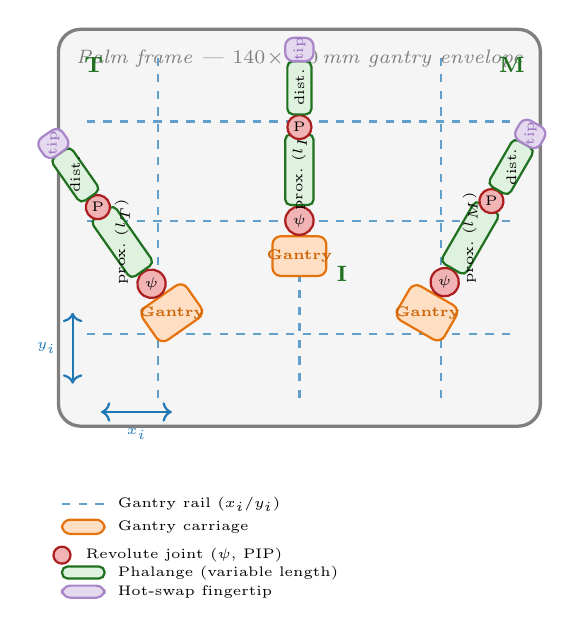
\begin{tikzpicture}[scale=0.90, font=\small,
  rail/.style={draw=mblue!70, thick, dashed},
  finger/.style={draw=mgreen!70!black, fill=mgreen!15, rounded corners=2pt, thick},
  joint/.style={draw=mred!80!black, fill=mred!35, circle, inner sep=2pt, thick},
  act/.style={draw=morange!90!black, fill=morange!25, rounded corners=3pt, thick},
  tip/.style={draw=mpurple!80, fill=mpurple!25, rounded corners=3pt, thick},
  arrow/.style={-Stealth, thick, mblue}]

  % Palm boundary
  \draw[draw=mgray, fill=mgray!8, rounded corners=8pt, very thick]
    (-3.4,-2.6) rectangle (3.4, 3.0);
  \node[font=\scriptsize\itshape, mgray, anchor=north] at (0, 2.85)
    {Palm frame — $140\!\times\!100$\,mm gantry envelope};

  % Grid of rails (X and Y)
  \foreach \x in {-2.0, 0, 2.0}
    \draw[rail] (\x, -2.2) -- (\x, 2.6);
  \foreach \y in {-1.3, 0.3, 1.7}
    \draw[rail] (-3.0, \y) -- (3.0, \y);

  % ── THUMB ── lower-left, angled inward 35°
  \begin{scope}[shift={(-1.8, -1.0)}, rotate=35]
    \draw[act] (-0.38,-0.28) rectangle (0.38,0.28);
    \node[font=\tiny\bfseries, morange!80!black] at (0,0) {Gantry};
    % yaw joint
    \draw[joint] (0, 0.50) circle (0.20);
    \node[font=\tiny] at (0,0.50) {$\psi$};
    % proximal
    \draw[finger] (-0.20, 0.72) rectangle (0.20, 1.72);
    \node[font=\tiny, rotate=90] at (0, 1.22) {prox.\ ($l_T$)};
    % PIP joint
    \draw[joint] (0, 1.82) circle (0.17);
    \node[font=\tiny] at (0,1.82) {P};
    % distal
    \draw[finger] (-0.17, 2.00) rectangle (0.17, 2.75);
    \node[font=\tiny, rotate=90] at (0, 2.38) {dist.};
    % fingertip
    \draw[tip] (-0.20, 2.75) rectangle (0.20, 3.08);
    \node[font=\tiny, mpurple, rotate=90] at (0, 2.92) {tip};
  \end{scope}
  \node[font=\footnotesize\bfseries, mgreen!70!black] at (-2.9, 2.5) {T};

  % ── INDEX ── center, upright
  \begin{scope}[shift={(0, -0.2)}, rotate=0]
    \draw[act] (-0.38,-0.28) rectangle (0.38,0.28);
    \node[font=\tiny\bfseries, morange!80!black] at (0,0) {Gantry};
    \draw[joint] (0, 0.50) circle (0.20);
    \node[font=\tiny] at (0,0.50) {$\psi$};
    \draw[finger] (-0.20, 0.72) rectangle (0.20, 1.72);
    \node[font=\tiny, rotate=90] at (0, 1.22) {prox.\ ($l_I$)};
    \draw[joint] (0, 1.82) circle (0.17);
    \node[font=\tiny] at (0,1.82) {P};
    \draw[finger] (-0.17, 2.00) rectangle (0.17, 2.75);
    \node[font=\tiny, rotate=90] at (0, 2.38) {dist.};
    \draw[tip] (-0.20, 2.75) rectangle (0.20, 3.08);
    \node[font=\tiny, mpurple, rotate=90] at (0, 2.92) {tip};
  \end{scope}
  \node[font=\footnotesize\bfseries, mgreen!70!black] at (0.6, -0.45) {I};

  % ── MIDDLE ── right, angled inward -30°
  \begin{scope}[shift={(1.8, -1.0)}, rotate=-30]
    \draw[act] (-0.38,-0.28) rectangle (0.38,0.28);
    \node[font=\tiny\bfseries, morange!80!black] at (0,0) {Gantry};
    \draw[joint] (0, 0.50) circle (0.20);
    \node[font=\tiny] at (0,0.50) {$\psi$};
    \draw[finger] (-0.20, 0.72) rectangle (0.20, 1.72);
    \node[font=\tiny, rotate=90] at (0, 1.22) {prox.\ ($l_M$)};
    \draw[joint] (0, 1.82) circle (0.17);
    \node[font=\tiny] at (0,1.82) {P};
    \draw[finger] (-0.17, 2.00) rectangle (0.17, 2.75);
    \node[font=\tiny, rotate=90] at (0, 2.38) {dist.};
    \draw[tip] (-0.20, 2.75) rectangle (0.20, 3.08);
    \node[font=\tiny, mpurple, rotate=90] at (0, 2.92) {tip};
  \end{scope}
  \node[font=\footnotesize\bfseries, mgreen!70!black] at (3.0, 2.5) {M};

  % ── DOF annotation arrows ──
  \draw[arrow, <->] (-3.2, -2.0) -- (-3.2, -1.0);
  \node[left, font=\tiny, mblue] at (-3.3, -1.5) {$y_i$};
  \draw[arrow, <->] (-2.8, -2.4) -- (-1.8, -2.4);
  \node[below, font=\tiny, mblue] at (-2.3, -2.5) {$x_i$};

  % ── Legend ──
  \begin{scope}[shift={(-3.35, -3.7)}]
    \draw[rail] (0,0) -- (0.6,0);
    \node[right, font=\tiny] at (0.65, 0) {Gantry rail ($x_i$/$y_i$)};
    \draw[act] (0,-0.42) rectangle (0.6,-0.22);
    \node[right, font=\tiny] at (0.65,-0.32) {Gantry carriage};
    \draw[joint] (0,-0.72) circle (0.12);
    \node[right, font=\tiny] at (0.2,-0.72) {Revolute joint ($\psi$, PIP)};
    \draw[finger] (0,-1.05) rectangle (0.6,-0.88);
    \node[right, font=\tiny] at (0.65,-0.97) {Phalange (variable length)};
    \draw[tip] (0,-1.32) rectangle (0.6,-1.15);
    \node[right, font=\tiny] at (0.65,-1.24) {Hot-swap fingertip};
  \end{scope}

\end{tikzpicture}
\caption{%
Schematic top-down view of the MorphoHand palm (not to scale).
Three fingers T (thumb), I (index), M (middle) each mount on an independent XY gantry
(dashed grid lines show rail extent).
The yaw joint $\psi_i$ at each base controls finger splay.
Proximal phalange length $l_i$ is variable via an internal linear actuator.
The distal segment terminates in a hot-swap fingertip mount.
Annotation arrows indicate the $x_i$ (lateral) and $y_i$ (fore-aft) gantry DOFs.
The default configuration shown has T and M angled inward for a convergent grasp
posture; the optimizer may discover configurations with very different triangulations.}
\label{fig:schematic}
\end{figure}

% ============================================================
\section{Simulation and Optimization Pipeline}
\label{sec:sim}
% ============================================================

\subsection{Overview of the Pipeline}

The simulation pipeline has three nested levels:
\begin{enumerate}
  \item \textbf{Object library}: a fixed set of 3D object meshes with precomputed
    contact region libraries (Section~\ref{sec:objects}).
  \item \textbf{Inner loop (grasp synthesis)}: given a morphology $\btheta$ and an object,
    find the joint angles $\bq$ that maximize the GWS epsilon metric
    (Section~\ref{sec:inner}).
  \item \textbf{Outer loop (morphology search)}: use MAP-Elites to propose and evaluate
    morphology configurations, building an archive of diverse high-quality morphologies
    (Section~\ref{sec:outer}).
\end{enumerate}
These levels are composed to produce the simulation output: an archive mapping
morphology configurations to grasp quality, one archive per object distribution.

\subsection{MJCF Model Parameterization}

MorphoHand's 3-finger kinematics are encoded as a MuJoCo MJCF model with 18 actuated
joints.
The morphological parameters $\btheta$ are instantiated via template substitution:
a Python script generates a new MJCF file for each $\btheta$ by substituting the
gantry positions, yaw angles, and phalange lengths into the XML template.
Batches of morphologies are instantiated as separate MuJoCo worlds run in parallel
(via MJX or MJWarp, depending on whether gradients are needed).

Contact site arrays are defined on the distal segment and proximal phalange surface
at multiple locations, enabling measurement of contact wrenches at each potential
contact point independently.

\subsection{Grasp Wrench Space Metric Implementation}

For a grasp with $n$ contact points at positions $\mathbf{p}_j$, each with contact
normal $\hat{\mathbf{n}}_j$ and friction coefficient $\mu_j$, the contact wrench
primitive at contact $j$ for force direction $\hat{\mathbf{f}}$ within the friction cone is:
\begin{equation}
  \bw_j(\hat{\mathbf{f}}) = G_j \hat{\mathbf{f}}, \quad
  G_j = \begin{bmatrix} I \\ [\mathbf{p}_j]_\times \end{bmatrix} \in \R^{6\times 3},
  \label{eq:wrench_primitive}
\end{equation}
where $G_j$ is the grasp map for contact $j$ and $[\mathbf{p}_j]_\times$ is the
cross-product matrix.
The GWS is the Minkowski sum of the friction-cone-scaled wrench primitives across all contacts:
\begin{equation}
  \text{GWS} = \bigoplus_{j=1}^n \mathrm{conv}\!\left(\left\{G_j \hat{\mathbf{f}} : \|\hat{\mathbf{f}} - \hat{\mathbf{n}}_j\| \leq \mu_j\right\}\right).
  \label{eq:gws}
\end{equation}
The epsilon metric is the radius of the inscribed ball:
\begin{equation}
  \eps(\btheta, \bq) = \min_{\|\bw\|_2 = 1}\; \sigma_{\text{GWS}}(\bw),
  \label{eq:eps}
\end{equation}
where $\sigma_{\text{GWS}}(\bw)$ is the support function of the GWS evaluated in direction $\bw$.

We implement the GWB differentiable approximation~\cite{gwb2023}: rather than computing
the exact convex hull (NP-hard in 6D), we sample a large number of wrench directions
uniformly on the 6D unit sphere, compute the support in each direction via parallelized
GPU sampling, and return the minimum support as the epsilon estimate.
This runs in milliseconds on GPU and provides accurate gradients via automatic
differentiation in JAX.

\subsection{Inner Loop: Contact-Map-Guided Grasp Synthesis}
\label{sec:inner}

\subsubsection{Contact Region Library}

For each object in the benchmark, we precompute a library of candidate contact regions.
A contact region is a patch of the object surface that, if contacted by a fingertip,
contributes positively to force closure.
Contact regions are computed by:
\begin{enumerate}
  \item Sampling $10^4$ random contact point triples on the object surface;
  \item For each triple, computing the GWS epsilon assuming point contacts with friction
    $\mu = 0.5$;
  \item Retaining the top-$K = 200$ triples as candidate contact configurations;
  \item Clustering the retained triples into regions using DBSCAN to remove near-duplicates.
\end{enumerate}
This produces a small library of 10--30 canonical contact configurations per object,
each associated with an expected GWS epsilon value.

\subsubsection{FK Feasibility Check and IK Initialization}

For a given morphology $\btheta$, the inner optimizer selects the contact configuration
$\mathcal{C}^*$ from the library that is most reachable by the current finger kinematics.
Reachability is estimated by a fast forward kinematics (FK) check: for each candidate
contact configuration, compute the minimum joint-space distance between the FK-predicted
fingertip positions (over the joint angle space $\cQ(\btheta)$) and the target contact
positions.
The configuration with minimum distance is selected, and IK is run to find the initial
$\bq_0$ that places fingertips at (or near) the target contact points.

\subsubsection{Gradient Ascent on $\eps$}

Starting from $\bq_0$, gradient ascent on the differentiable GWS epsilon is run:
\begin{equation}
  \bq_{t+1} = \bq_t + \alpha \nabla_{\bq} \eps(\btheta, \bq_t),
  \label{eq:gradascent}
\end{equation}
with step size $\alpha$ controlled by an Adam optimizer, for a fixed number of steps
(typically 200--500 iterations in our preliminary experiments).
The CFD augmentation~\cite{diffmjx2025} ensures that gradients are informative even
when fingers are not yet in contact with the object.
Joint limits $\cQ(\btheta)$ are enforced via projected gradient.

The output is the optimized $\bq^*(\btheta)$ and the achieved quality
$\eps(\btheta, \bq^*(\btheta))$.

\subsection{Outer Loop: MAP-Elites Morphology Search}
\label{sec:outer}

\subsubsection{Archive Structure and Behavioral Descriptors}

The archive is a $B \times B$ grid (default $B = 20$, yielding $400$ cells) indexed by
two behavioral descriptors computed from the optimal grasp configuration:
\begin{align}
  \bar{s}(\btheta, \bq^*) &= \frac{1}{\binom{3}{2}} \sum_{i \neq j}
    \|\mathbf{f}_i(\btheta, \bq^*) - \mathbf{f}_j(\btheta, \bq^*)\|_2,
  \label{eq:spread} \\
  \bar{r}(\btheta, \bq^*) &= \frac{1}{3} \sum_i
    \|\mathbf{f}_i(\btheta, \bq^*) - \bar{\mathbf{f}}\|_2,
  \label{eq:reach}
\end{align}
where $\mathbf{f}_i(\btheta, \bq^*)$ is the fingertip position of finger $i$ at the
optimal grasp, and $\bar{\mathbf{f}}$ is the palm centroid.
$\bar{s}$ is the mean fingertip spread (captures how widely the hand opens); $\bar{r}$
is the mean palm-normalized reach (captures how far the hand extends).
These two descriptors are:
\begin{itemize}
  \item \textbf{Interpretable}: they correspond directly to recognizable aspects of hand
    shape (compact/spread, close/extended).
  \item \textbf{Hardware-measurable}: they can be computed from joint encoder readings
    on the physical platform, enabling direct comparison between simulation and hardware
    descriptor values.
  \item \textbf{Orthogonal}: fingers can be spread but short (wide flat object grasp),
    or converged but long (narrow deep object), making the 2D descriptor grid meaningful.
\end{itemize}

\subsubsection{MAP-Elites Algorithm}

\begin{algorithm}
\caption{MAP-Elites for Morphology Optimization}
\label{alg:mapelites}
\begin{algorithmic}[1]
\REQUIRE Object distribution $\cO$, bounds $\Theta$, inner-loop oracle $\eps(\cdot)$
\ENSURE Archive $\cA$ of elite morphologies
\STATE Initialize $\cA \leftarrow \emptyset$
\STATE Sample $N_{\text{init}}$ morphologies $\{\btheta_k\}$ via Latin hypercube over $\Theta$
\FOR{each $\btheta_k$}
  \STATE Evaluate $q_k = \mathbb{E}_{o \sim \cO}[\eps(\btheta_k, \bq^*(\btheta_k, o))]$
  \STATE Compute descriptors $(s_k, r_k)$
  \STATE Update archive: $\cA[s_k, r_k] \leftarrow \btheta_k$ if $q_k > \cA[s_k, r_k].q$
\ENDFOR
\FOR{$t = 1, \ldots, N_{\text{iter}}$}
  \STATE Sample parent $\btheta_p$ uniformly from occupied cells of $\cA$
  \STATE Generate offspring $\btheta' = \btheta_p + \mathcal{N}(0, \sigma^2 I)$
  \STATE Project $\btheta'$ to $\Theta$
  \IF{surrogate $\hat{q}(\btheta') > q_{\text{thresh}}$}
    \STATE Evaluate $q' = \mathbb{E}_{o \sim \cO}[\eps(\btheta', \bq^*(\btheta', o))]$ (full oracle)
    \STATE Compute descriptors $(s', r')$
    \STATE Update archive: $\cA[s', r'] \leftarrow \btheta'$ if $q' > \cA[s', r'].q$
    \STATE Update surrogate with $(\btheta', q')$
  \ENDIF
\ENDFOR
\RETURN $\cA$
\end{algorithmic}
\end{algorithm}

The surrogate prescreening step (line 12) uses a Gaussian process trained on
all previously evaluated morphologies.
Only offspring whose predicted quality exceeds the $p$-th percentile of current archive
qualities (default $p = 0.5$) are passed to the full oracle.
This halves the number of expensive inner-loop calls without measurably degrading archive
quality, consistent with results from SAIL~\cite{gaier2017sail}.

\subsubsection{Multi-Object Evaluation}

For each morphology proposal, the inner loop is run on a mini-batch of $K = 10$ objects
drawn from $\cO$.
The quality estimate is the mean epsilon across the batch:
\begin{equation}
  q(\btheta) = \frac{1}{K} \sum_{k=1}^K \eps(\btheta, \bq^*(\btheta, o_k)).
  \label{eq:quality}
\end{equation}
Using a batch rather than the full object set reduces evaluation cost while still
capturing the distributional character of the quality function.
Batch size $K$ can be increased for final evaluation of archive elites.

\subsection{Gradient Augmentation via CMA-ME}
\label{sec:cmame}

In regions of the archive where the contact set is stable (the same fingers are in contact
before and after a morphology perturbation), gradients of quality with respect to $\btheta$
can be computed by differentiating the inner-loop objective through the FK:
\begin{equation}
  \frac{d\eps}{d\btheta} = \frac{\partial \eps}{\partial \bq^*}
  \cdot \frac{\partial \bq^*}{\partial \btheta}
  + \frac{\partial \eps}{\partial \btheta}\bigg|_{\bq^*}.
  \label{eq:morphgrad}
\end{equation}
The first term requires differentiating the inner-loop IK through $\btheta$ (available
from MJX's differentiable FK).
The second term captures the direct effect of morphology on the grasp wrench (e.g.,
longer phalange $\to$ different contact normal $\to$ different wrench direction).
Both are available from the JAX autodiff tape of the inner-loop optimization.

When these gradients are reliable (estimated via the gradient norm being large compared
to noise), we use a gradient-augmented MAP-Elites variant (following CMA-MAEGA~\cite{cmamae2022})
that generates offspring by taking a gradient step in morphology space rather than random
Gaussian mutation.
When gradients are not reliable (near contact-mode boundaries, or when the inner-loop
optimizer changed contact configuration between $\btheta$ and $\btheta'$), we fall back
to standard Gaussian mutation.

\subsection{Simulation Stack Summary}

\begin{table}[t]
  \centering
  \caption{Simulation Stack Components and Their Roles}
  \label{tab:simstack}
  \resizebox{\columnwidth}{!}{%
  \begin{tabular}{lll}
    \toprule
    \textbf{Component} & \textbf{Tool} & \textbf{Role} \\
    \midrule
    Physics simulator & MJX (JAX) & Differentiable inner-loop dynamics \\
    Parallel sampling & MJWarp / Isaac Lab & Non-diff.\ batch morphology evaluation \\
    Future unified & Newton & Diff.\ + parallel (when mature) \\
    GWS metric & GWB estimator~\cite{gwb2023} & Inner-loop quality oracle (ms/GPU) \\
    Contact gradients & DiffMJX CFD~\cite{diffmjx2025} & Pre-contact gradient signal \\
    Outer optimizer & MAP-Elites + CMA-MAEGA & Archive construction \\
    Surrogate & Gaussian process (SAIL~\cite{gaier2017sail}) & Pre-screen candidates \\
    MJCF generation & Python templating & Batch morphology instantiation \\
    \bottomrule
  \end{tabular}}
\end{table}

% ============================================================
\section{Object Set and Grasp Benchmark}
\label{sec:objects}
% ============================================================

\subsection{Design Principles for the Object Set}

A good object set for morphology evaluation must:
\begin{enumerate}
  \item Be diverse enough to differentiate morphologies: if all objects prefer the same
    contact triangulation, no morphology specificity will be observed.
  \item Be physically realizable: objects must exist in the real world and be poseable
    repeatably on the hardware platform.
  \item Span known geometric extremes: compact, elongated, flat, and irregular objects
    each stress different aspects of hand morphology.
  \item Be available as 3D meshes for simulation: either from the YCB dataset~\cite{ycb2017}
    or custom-designed.
\end{enumerate}

\subsection{Object Clusters}

We assemble 40 objects across four geometric clusters:

\begin{table}[t]
  \centering
  \caption{Object Benchmark Clusters}
  \label{tab:objects}
  \resizebox{\columnwidth}{!}{%
  \begin{tabular}{lllp{3.5cm}}
    \toprule
    \textbf{Cluster} & \textbf{Name} & \textbf{Count} & \textbf{Geometric character} \\
    \midrule
    A & Compact / symmetric & 10 & Spheres, cubes 30--80\,mm; prefer enveloping \\
    B & Elongated / cylindrical & 10 & Cylinders, prisms $\varnothing$20--40\,mm $\times$ 80--150\,mm; prefer wide spread \\
    C & Flat / planar & 10 & Discs, tablets 2--10\,mm height; prefer low clearance approach \\
    D & Irregular / YCB & 10 & Banana, mug, hammer, scissors (YCB subset); prefer task-specific triangulation \\
    \bottomrule
  \end{tabular}}
\end{table}

The object set is designed so that the optimal contact triangulation differs substantially
between clusters: Cluster A prefers a nearly equilateral fingertip triangle centered on
the object; Cluster B prefers two fingers on one side and one on the other (power cylinder
grasp); Cluster C requires fingers to approach nearly flat and close with minimal palm
clearance; Cluster D has object-specific requirements that may not be captured by any
single simple grasp heuristic.
If the object-set specificity hypothesis is correct, the MAP-Elites archive should have
different high-quality regions for each cluster.

\subsection{Contact Region Library Computation}

For each object, contact region computation (Section~\ref{sec:inner}) is run offline
on the full set of $10^4$ candidate contact triples.
This is a one-time cost per object.
The library is stored and reused for all morphology evaluations involving that object.

\subsection{Physical Experimental Protocol}

On hardware, grasp success is evaluated via the \emph{shake test}:
\begin{enumerate}
  \item MorphoHand is configured to morphology $\btheta$ via gantry, yaw, and length
    actuators.
  \item The robot arm presents the hand in the approach orientation predicted by the
    simulation as optimal for the given object and morphology.
  \item The hand closes to joint angles $\bq^*(\btheta)$ as found by the inner optimizer.
  \item The arm lifts the object 20\,cm.
  \item The arm executes a predefined 6-DOF perturbation trajectory (3 translational
    shakes $\pm$5\,cm, 3 rotational shakes $\pm$20$^\circ$, each at 0.2\,m/s).
  \item Success is recorded if the object remains in hand after the full trajectory.
  \item Wrist F/T data are logged throughout for continuous quality analysis.
\end{enumerate}
Five trials per (morphology, object) pair are run.
Binary success rate (0--5 successes out of 5 trials) is the primary hardware quality metric.
Minimum wrist-measured grasp wrench magnitude over the perturbation trajectory is the
continuous quality proxy for correlation with $\eps$.

% ============================================================
\section{Experimental Methodology}
\label{sec:experiments}
% ============================================================

\subsection{Experiment 1: Sim-to-Real Rank Correlation}

\subsubsection{Goal}
Establish whether simulation-predicted morphology rankings transfer to hardware.
This is the foundational validity check for the entire pipeline: if simulation rankings
do not correlate with hardware outcomes, the optimization results cannot be trusted for
hardware guidance.

\subsubsection{Protocol}
\begin{enumerate}
  \item Run MAP-Elites for $N_{\text{iter}} = 2000$ outer iterations over $\cO_{\text{all}}$.
  \item Extract the top-$M = 30$ archive elites by quality, subject to the constraint
    that selected morphologies span at least $M/2$ distinct archive cells (ensuring diversity).
  \item For each of the $M$ morphologies, command MorphoHand to the target $\btheta$ via
    gantry, yaw, and length actuators.
    Record the \emph{realized} morphology by reading back the servo positions and computing
    the actual FK, noting any deviation from the commanded $\btheta$.
  \item Run the physical shake-test protocol on all 40 objects $\times$ 5 trials for
    each of the $M$ morphologies.
  \item Compute the simulation quality rank and the hardware success-rate rank for each
    morphology. Compute Kendall's $\tau$ rank correlation.
\end{enumerate}

\subsubsection{Expected Outcome and Failure Analysis}
We target $\tau > 0.7$.
Values between 0.5 and 0.7 would indicate moderate correlation, motivating simulation
model refinement.
Values below 0.5 would constitute evidence that the sim-to-real gap for morphology is
substantial.
A post-hoc analysis of the largest ranking discrepancies would identify which morphological
features (e.g., extreme yaw angles, minimum phalange length) are most poorly modeled.

\subsection{Experiment 2: Object-Set Specificity}

\subsubsection{Goal}
Test the central hypothesis: the morphology that is optimal for the full object set is
not optimal for each subset, and the optimal morphology differs between subsets.

\subsubsection{Protocol}
\begin{enumerate}
  \item Run MAP-Elites separately over $\cO_{\text{all}}, \cO_A, \cO_B, \cO_C, \cO_D$
    (five runs, same number of iterations).
  \item Extract the top-1 elite from each archive:
    $\btheta^*_{\text{all}}, \btheta^*_A, \btheta^*_B, \btheta^*_C, \btheta^*_D$.
  \item Cross-evaluate: compute $q(\btheta^*_k, \cO_j)$ for all pairs $(k, j)$ in simulation,
    producing a $5\times5$ quality matrix.
  \item Compute the specialization ratio for each pair:
    \begin{equation}
      SR_{k \to j} = \frac{q(\btheta^*_k, \cO_j)}{q(\btheta^*_j, \cO_j)},
      \label{eq:sr}
    \end{equation}
    where $SR_{j \to j} = 1$ by definition and $SR_{k \to j} \leq 1$ for $k \neq j$
    if the cluster-specific optimal is always better on its own cluster.
  \item Physically validate the top-1 elite from each archive on all five object
    distributions using the shake test (5 morphologies $\times$ 5 distributions
    $\times$ 40 objects $\times$ 5 trials = 5,000 trials total).
  \item Compare the hardware specialization ratios with the simulation specialization
    ratios.
\end{enumerate}

\subsubsection{Expected Outcome}
We expect $SR_{\text{all} \to j} < 0.90$ for at least 3 of 4 clusters,
with the flattest objects (Cluster C) showing the largest specialization gap because
flat object grasping requires the most distinctive morphology (low approach clearance,
high MCP extension, thumb repositioned far forward).

\subsection{Experiment 3: Archive Coverage and Surrogate Efficiency}

\subsubsection{Goal}
Characterize how densely MAP-Elites explores the achievable descriptor space, and whether
surrogate-assisted illumination reduces compute without degrading the archive.

\subsubsection{Protocol}
Compare four outer-loop variants over $\cO_{\text{all}}$:
(a) Vanilla MAP-Elites (random Gaussian mutation, no surrogate, no gradients);
(b) MAP-Elites + GP surrogate (SAIL~\cite{gaier2017sail});
(c) CMA-ME (covariance-matrix-adapted mutation, no surrogate);
(d) CMA-MAEGA (gradient-augmented, with surrogate).
Metrics: archive coverage (\% cells occupied), mean elite quality, QD-score
($= \sum_{\text{cells}} q_{\text{cell}}$), and wall-clock time to achieve 90\% of the
asymptotic QD-score.

\subsection{Experiment 4: Morphological DOF Contribution}

\subsubsection{Goal}
Quantify the individual contribution of each morphological DOF class to the achievable
quality range.

\subsubsection{Protocol}
Run MAP-Elites with one DOF class held fixed at its default value at a time:
\begin{itemize}
  \item \textbf{No gantry} ($x_i = y_i = 0$): fingers start at the default mounting positions.
  \item \textbf{No yaw} ($\psi_i = 0$): fingers always point perpendicular to palm.
  \item \textbf{No length variation} ($l_i = 65$\,mm mid-range): phalange length fixed.
  \item \textbf{Fully fixed morphology}: all morphological DOFs at defaults
    (baseline comparable to a conventional fixed-geometry hand).
\end{itemize}
Compare the QD-score and top-1 quality of each ablation against the full 12-DOF optimizer.
This directly quantifies the marginal value of each hardware design choice.

\subsection{Experiment 5: Hardware Repeatability}

\subsubsection{Goal}
Characterize the mechanical repeatability of MorphoHand: given the same commanded $\btheta$,
how consistently does the platform instantiate the morphology across multiple re-configurations?

\subsubsection{Protocol}
Select 5 morphologies spanning the descriptor space.
For each, configure the platform, run 5 grasp trials on a single test object, then
fully reconfigure to a different morphology and return.
Repeat this reconfiguration cycle 10 times per morphology.
Record the realized morphology (FK from servo encoder readings) and grasp success for
each trial.
Compute the standard deviation of realized morphology parameters across cycles as a
repeatability metric.
Acceptable repeatability: $\sigma_{x,y} < 1$\,mm, $\sigma_\psi < 1^\circ$,
$\sigma_l < 1$\,mm.

% ============================================================
\section{Discussion}
\label{sec:discussion}
% ============================================================

\subsection{Expected Results and Their Interpretation}

\subsubsection{On Rank Correlation (Exp.\ 1)}

A correlation of $\tau > 0.7$ would indicate that the simulation pipeline is a reliable
proxy for hardware performance, validating the use of simulation for morphology search.
It would also mean that the GWS epsilon metric---despite its simplified contact model---is
a good predictor of real-world grasp stability in the quasi-static regime.

Lower correlations would reveal which aspects of the simulation are most unrealistic.
Our expectation is that the main sources of discrepancy will be:
\begin{itemize}
  \item \textbf{Mechanical compliance}: the telescoping phalange actuator and gantry
    are not perfectly rigid; real contacts may differ from simulated ones due to small
    deflections.
  \item \textbf{Friction variation}: rubber fingertips have direction-dependent and
    velocity-dependent friction not captured by isotropic Coulomb friction.
  \item \textbf{Sim-to-real morphology error}: the realized $\btheta$ (from servo readings)
    may differ slightly from the commanded $\btheta$ due to mechanical play.
\end{itemize}
All three effects can be characterized and partially compensated by system identification:
measuring the actual stiffness and friction properties of the physical system and
updating the MJCF model accordingly.

\subsubsection{On Object-Set Specificity (Exp.\ 2)}

The interesting result is not merely that specificity exists, but \emph{by how much} and
\emph{which morphological parameters are responsible}.
A strong result would show that the optimal morphologies for Clusters B and C differ by
more than one standard deviation in gantry position or phalange length, and that this
difference is replicated on hardware.
A weak result (all cluster-optimal morphologies are similar) would suggest that for
\emph{3-finger hands}, the design space is not rich enough to meaningfully specialize to
these object clusters---an equally important negative result.

\subsubsection{On the Design Space (Exp.\ 4)}

The DOF contribution experiment tests a practical question that matters for future hardware
design: if you were to build a simpler version of MorphoHand, which DOF class would you
keep?
We predict that the gantry position ($x_i, y_i$) contributes most, because it controls
the shape of the contact triangle---the single most important geometric factor in
force-closure quality.
Yaw ($\psi_i$) contributes next because it controls the direction of applied force.
Phalange length ($l_i$) contributes the least because its effect is largely captured by
gantry position (moving the finger base closer approximates a shorter phalange for many
objects).

\subsection{Limitations}

\subsubsection{Quasi-Static Restriction}

All experiments are quasi-static: the platform was not designed for dynamic grasping
or in-hand manipulation.
This is a principled restriction (GWS metrics are most meaningful in this regime)
but means the results do not directly address dynamic manipulation scenarios.
The optimal morphology for dynamic in-hand manipulation (where inertia and velocity
matter) may differ from the static optimal.

\subsubsection{3-Finger Topology Only}

We fix the number of fingers (three) and the phalange topology (two per finger).
The platform cannot explore topologies with more fingers, asymmetric phalange counts,
or prismatic joints.
These are meaningful restrictions on the morphology space.
Future work could extend MorphoHand to four fingers or variable phalange count.

\subsubsection{Fingertip Contact Model}

We use flat silicone pads throughout.
The contact mechanics of silicone pads (material compliance, direction-dependent friction,
adhesion) are not fully captured by the Coulomb friction model.
Future work should incorporate a more accurate fingertip contact model in simulation
and characterize the real fingertip properties.

\subsubsection{Object Set Size}

40 objects is a manageable set for hardware evaluation but is small relative to the
diversity of real-world manipulation tasks.
The geometric clusters are coarse.
Future work should expand to a larger, more systematically constructed object set
(e.g., ShapeNet subsets with controlled geometry variation).

\subsection{Open Questions}

This proposal leaves several questions explicitly open for future work:
\begin{itemize}
  \item \textbf{What is the right behavioral descriptor for the MAP-Elites archive?}
    Fingertip spread and palm reach are interpretable and hardware-measurable, but other
    descriptors (contact area, approach angle diversity) might better correlate with
    object-set performance.
  \item \textbf{How does the optimal morphology scale with object size distribution?}
    If all objects in the set are twice as large, does the optimal morphology simply
    scale linearly, or are there nonlinear effects?
  \item \textbf{Can we recover the sim-to-real gap through system identification?}
    If the rank correlation (Exp.\ 1) is low, can we measure the physical system
    properties and update the MJCF model to improve it?
  \item \textbf{Is the reconfigurable platform useful for policy learning, not just
    morphology evaluation?}
    Given a fixed morphology found by the optimizer, the platform can also be used to
    collect demonstration data or to test RL policies without re-fabricating a hand.
\end{itemize}

% ============================================================
\section{Conclusion}
\label{sec:conclusion}
% ============================================================

We have presented MorphoHand, a proposal for an 18-DOF reconfigurable robotic hand
platform designed as a physical oracle for simulation-based morphology optimization.
The platform's defining feature is that all major morphological parameters---finger
base XY position via Cartesian gantry, yaw, proximal phalange length, and joint angles---are
motorized and programmable, enabling dense in-session evaluation of the morphology
design space without disassembly or re-fabrication.

On the simulation side, we propose a MAP-Elites quality-diversity pipeline using a
differentiable Grasp Wrench Space metric as the inner oracle and surrogate-assisted
illumination to reduce evaluation cost.
The pipeline produces archives that illuminate how grasp quality varies across the full
morphology design space for a given object distribution---a representation that directly
enables the scientific question at the heart of this work: does the optimal 3-finger
hand morphology depend on the object distribution, and if so, by how much and through
which parameters?

This paper is explicitly presented as a working proposal.
The hardware has not yet been built; the simulation pipeline is partially implemented.
The experiments described in Section~\ref{sec:experiments} define the validation roadmap.
The expected results in Section~\ref{sec:discussion} make explicit, falsifiable predictions
that will determine whether the approach succeeds.

The broader contribution, if successful, is methodological: a workflow for morphology
validation that is not limited to a single fabricated hand, but that treats the physical
design space as something to be \emph{measured} rather than just guessed at.

% ============================================================
\bibliographystyle{IEEEtran}
\bibliography{references}
% ============================================================

\end{document}